\documentclass[10pt,conference]{IEEEtran}
\usepackage[utf8]{inputenc}
\usepackage{graphicx}
\usepackage[nocompress]{cite}
\usepackage{caption}
\usepackage{subcaption}

%\newcommand{\per}[1]{}
%\newcommand{\anna}[1]{}
%\newcommand{\kiran}[1]{}

% Title Page
\title{Probe or Wait: Handling tail losses using Multipath TCP}

\author{\IEEEauthorblockN{Kiran~Yedugundla, Per~Hurtig, Anna~Brunstrom}
\IEEEauthorblockA{Dept. of Computer Science, Karlstad University, Karlstad, Sweden\\
    \{name.surname\}@kau.se
}}

\IEEEoverridecommandlockouts
\IEEEpubid{%
   \makebox[\columnwidth]{ISBN 978-3-901882-94-4~\copyright~2017 IFIP \hfill}%
   \hspace{\columnsep}%
   \makebox[\columnwidth]{ }%
}

\begin{document}
\maketitle

\begin{abstract}
Packet losses are known to affect the performance of latency sensitive applications in the Internet such as media streaming and gaming. 
Transport protocols recover from packet loss in order to provide reliable end-to-end communication and improve user experience. The efficiency of 
loss recovery mechanisms influences the completion time of flows. In this paper we focus on state-of-the-art loss recovery mechanisms for TCP 
and Multipath TCP. We use controlled tail loss scenarios to evaluate the performance of loss recovery mechanisms, and based on the observations, 
we propose an enhanced tail loss recovery mechanism for Multipath TCP, to improve the loss recovery time. Our experiment results using Linux 
Multipath TCP implementation show consistent end to end latency performance improvement in considered scenarios. 
\end{abstract}

\section{Introduction}


Multipath TCP~(MPTCP)~\cite{rfc6824} is an experimental standard proposed as an extension to TCP. MPTCP allows devices with multiple interfaces to 
transmit data simultaneously on both interfaces, thereby improving the throughput of end-to-end connections. Using MPTCP, a connection can have 
multiple TCP subflows using different interfaces on different routes. Each TCP subflow imparts the functional behavior of a standard TCP flow. 

TCP has two mechanisms for detecting and recovering from packet losses: Fast Retransmit (FR) and Retransmission Timeout~(RTO)~\cite{Flach:2013}. 
Fast retransmit is triggered on receipt of a predecided number of duplicate acknowledgements, considering it as an indication of loss. In the case 
of RTO, a sender waits for the packet loss to trigger a timeout before retransmitting packet. During such a timeout, the sender cannot send any 
packets. However, with FR the out-of-order packets trigger duplicate acknowledgements. The sender can start retransmission of missing packets 
without waiting for timeout. For flows where there are sufficiently many packets to be transferred, FR is quicker than RTO in detecting and 
recovering packet loss. Fast retransmit coupled with fast recovery can send data outstanding when there is enough data to send in long flows. 
On the other hand, shorter flows more frequently depend on RTO for packet loss detection and recovery, thus incurring more latency. A single 
packet loss in a short flow may take many RTTs to detect and recover. This scenario is also applicable to the packets at the end of the flow 
(or tail), of a long flow. Although RTO is reliable even in tail loss recovery, it is not efficient in terms of recovery completion time. Tail 
losses are one of the major causes of end-to-end latency detoriation in modern networks~\cite{Flach:2013}. 


TCP Loss Probe (TLP)~\cite{Flach:2013} is a mechanism to detect and recover from tail losses by employing a loss probe packet for a timeout shorter
than the RTO. Probe timeout enables short flows to recover packet loss at the tail, by triggering FR. It assumes that other algorithms such as 
Early Retransmit~(ER)\cite{rfc5827} and Forward Acknowledgement~(FACK)~\cite{FACK} threshold based recovery are enabled. TLP is available in the Linux 
kernel and enabled by default. Further, evaluations in~\cite{Rajiullah:2015} show that TLP provides significant latency reductions for short 
flows with one to n-degree tail losses. 

 MPTCP connections start with one TCP flow to send data over, and may add more flows to the connection if configured to. MPTCP uses a connection 
 level congestion window as well as subflow level congestion windows for each subflow. Data is split across the flows and each data packet is 
 scheduled on one of the subflows based on the minimum RTT. Packet losses in each subflow are detected and recovered in a similar fashion as that of 
 TCP. Loss recovery can be conducted at different levels: the MPTCP connection level (meta level) and at subflow level. If the recovery is handled 
 at meta level, a lost packet may be rescheduled and retransmitted on the available subflow with the lowest RTT. If recovery is handled at the 
 subflow level, the packet must be retransmitted on the same subflow. An important part of loss recovery process at the subflow level is to follow 
 the TCP semantics and retransmit lost packets on the initial path of transfer. However, the MPTCP standard~\cite{rfc6824} does not specify exactly, 
 how the loss recovery should happen in the implementation and which subflow should retransmit the lost packets.


In this paper, we analyze the retransmission behavior of MPTCP in selected tail loss cases to identify the scope for improvement. We propose a 
change in the retransmission strategy of MPTCP to improve the latency performance. We provide related research on MPTCP retransmission mechanisms in 
Section~\ref{relwork}, and describe the experimental setup in Section~\ref{exsetup}. We discuss observations from the experiments on state 
of the art retransmission behavior of TCP and MPTCP in Section~\ref{disc}. Based on the observations, we propose an improvement to the current 
Linux implementation of TLP for MPTCP in Section~\ref{impr}. In Section~\ref{eval}, we provide an evaluation of the proposed TLP for MPTCP 
mechanism and conclude the paper in Section~\ref{conc}. Our experimental results indicate improvement in the performance of TLP by reducing 
recovery time in the event of tail losses.
 
%\kern-1em
\section{Background and Related Work}\label{relwork}

Retransmission schemes are of significant importance in achieving a low flow completion time. Several IETF RFCs such as SACK based 
recovery~\cite{rfc6675}, Limited Transmit~\cite{rfc3042} and Early Retransmission~\cite{rfc5827} have led to improved retransmission 
strategies for TCP. TLP is part of the various deployable loss recovery mechanisms proposed in~\cite{Flach:2013}, suggesting that current 
Linux TCP implementation provides room for improvement in several packet loss scenarios. 

In a TCP flow, sequence numbers are used to identify lost packets and retransmit them. MPTCP uses two levels of sequence numbers to support 
efficient data transfer, namely data sequence and TCP sequence. Data sequence numbers are for the end-to-end data transfer and TCP sequence 
numbers are for individual flow data sequence. There is an association between data sequence numbers and TCP sequence numbers within a subflow.  
A loss occurring in an individual TCP flow corresponds to a loss in end-to-end data. Multipath TCP, as an extension of TCP, uses the 
TCP retransmission mechanism. However, the interaction between the two levels makes the problem of retransmitting more challenging than in TCP. The dual sequence 
numbering enables MPTCP to respond to loss of packets by retransmitting the lost packets on an alternate path.  

The Linux implementation of MPTCP uses a set of retransmission heuristics to handle retransmissions. The data outstanding on a timed out subflow 
should be rescheduled for transmission on a different subflow using timeout as the indicator. Fast retransmit on a subflow will not trigger 
retransmission on another subflow. The target devices of MPTCP contain a degree of asymmetry in their interface characteristics such as 3G or 
4G vs WLAN, leading to flows with different delay characteristics. Significant delay differences in available paths can cause receive buffer 
limitations, as the receiver has to wait for the data sent on a slow path, while buffering the data on the fast path. In such cases, opportunistic 
retransmission~\cite{Costin} improves the latency by using fast path to retransmit the data sent on an another path. Authors in~\cite{fuso}, try 
to exploit the path diversity by quickly retransmitting on the fastest paths. Such quick retransmission comes with a cost of redundant packets as 
each individual TCP flow should retransmit always as well to follow TCP semantics. The MPTCP standard~\cite{rfc6824} suggests a more conservative 
approach. MPTCP is designed to exploit the multiple interfaces and often one or more of these could be wireless with completely different 
characteristics than that of wired interfaces. Authors in~\cite{Shin} argue that the calculation of RTO for MPTCP flows should include the 
interface characteristics to improve loss recovery time. 


%\subsection{Scope}\label{scope}

This paper analyzes the performance of state-of-the-art loss recovery mechanism for MPTCP and presents a case for improvement in the tail loss 
scenario. For understanding the loss recovery and retransmission policies in the MPTCP Linux implementation (version 0.91), we consider several specific 
cases of tail losses. We use the default settings of the Linux kernel. The Linux implementation of TCP is considered as the baseline TCP 
retransmission for implementation flexibility and availability of TLP support.

%\kern-1em
\section{Experimental Setup}\label{exsetup}
\begin{figure}
\begin{center}
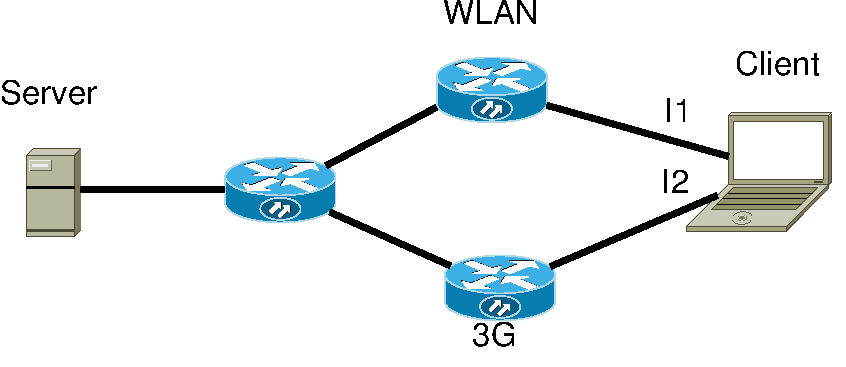
\includegraphics[angle=0, width=0.45\textwidth]{images/fortest.pdf}
\caption{Topology used for Emulation}\label{fig1}
\end{center}
\end{figure}

Experiments are run in the CORE emulation platform~\cite{CORE} with a simple topology as depicted in Figure~\ref{fig1}. The client node connect to two wireless interfaces 3G or 4G and WLAN and the server node connect to a wired router.
CORE uses the Linux networking stack in each node of the topology by using a lightweight virtualization technique known as Linux network namespaces.
Characteristics of the connection setup and assumptions about the parameters are provided in Table~\ref{tab1}.
There is no attempt in this study to focus on the effect of link specific characteristics in retransmission performance.

 
\begin{center}
    \begin{table}
\resizebox{0.45\textwidth}{!}{\begin{minipage}{0.45\textwidth}
\small
\begin{center}
\begin{tabular}{|c|cccccccccc|}
      \hline
      
      \multicolumn{1}{c}{} & & \\[\dimexpr-\normalbaselineskip-\arrayrulewidth]
      \textbf{Burst Size} & \multicolumn{10}{c|}{80 Packets} \\
      \hline
      \textbf{Separation Time} & \multicolumn{10}{c|}{2s} \\
      \hline

      \textbf{Oneway Delay} & \multicolumn{10}{c|}{20\,ms-120\,ms}  \\
      \hline 	
      \textbf{Bandwidth} & \multicolumn{10}{c|}{54Mbps}  \\
      \hline
      \textbf{Loss Model} & \multicolumn{10}{c|}{Deterministic}\\
      \hline
      	
\end{tabular}
\caption{Emulation parameters}\label{tab1}
\end{center}
\end{minipage}}
\end{table}
\end{center}

\begin{figure*}
 \begin{subfigure}{0.32\textwidth}
	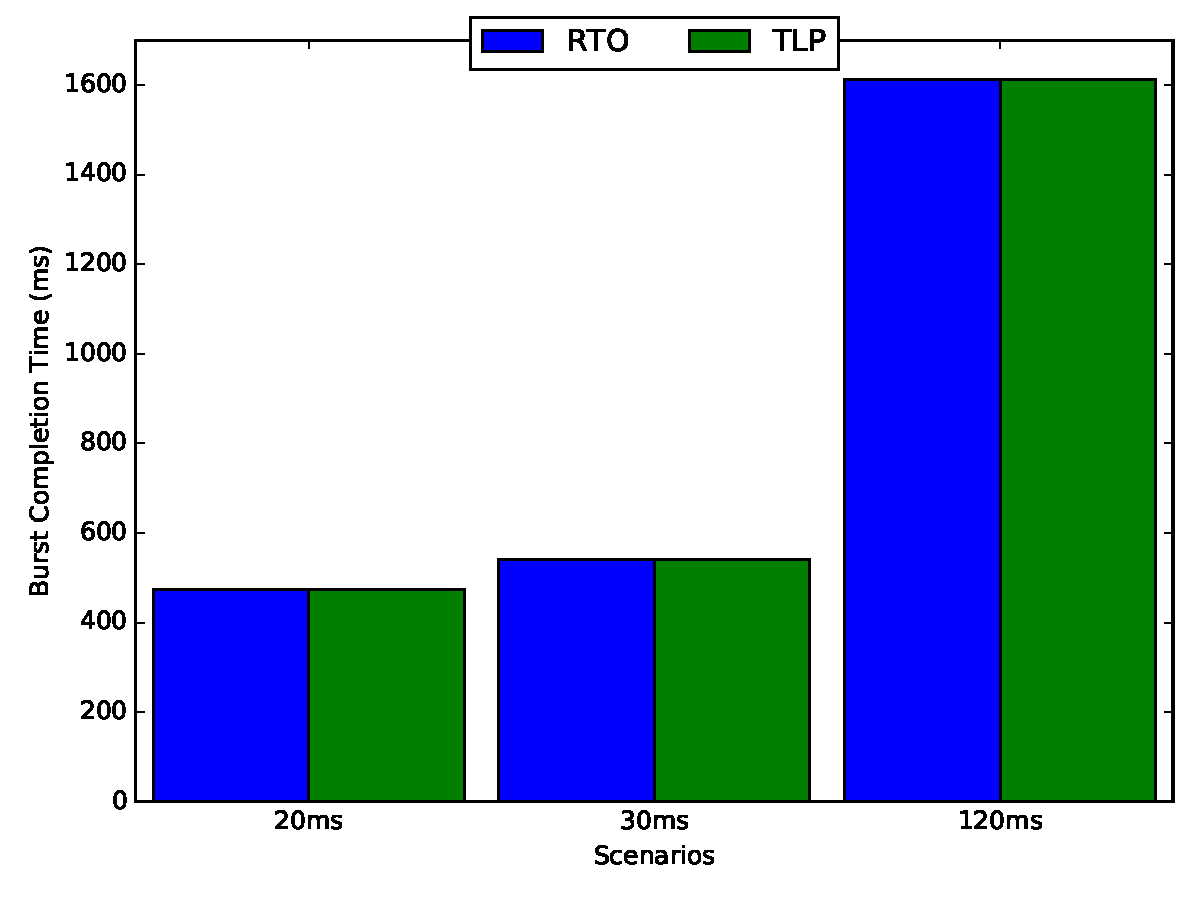
\includegraphics[angle=0, width=\textwidth,natwidth=578.16,natheight=433.62]{plots/T1P.pdf}
	\caption{Single packet}\label{t1p}
 \end{subfigure}
 \hfill
 \begin{subfigure}{0.32\textwidth}
	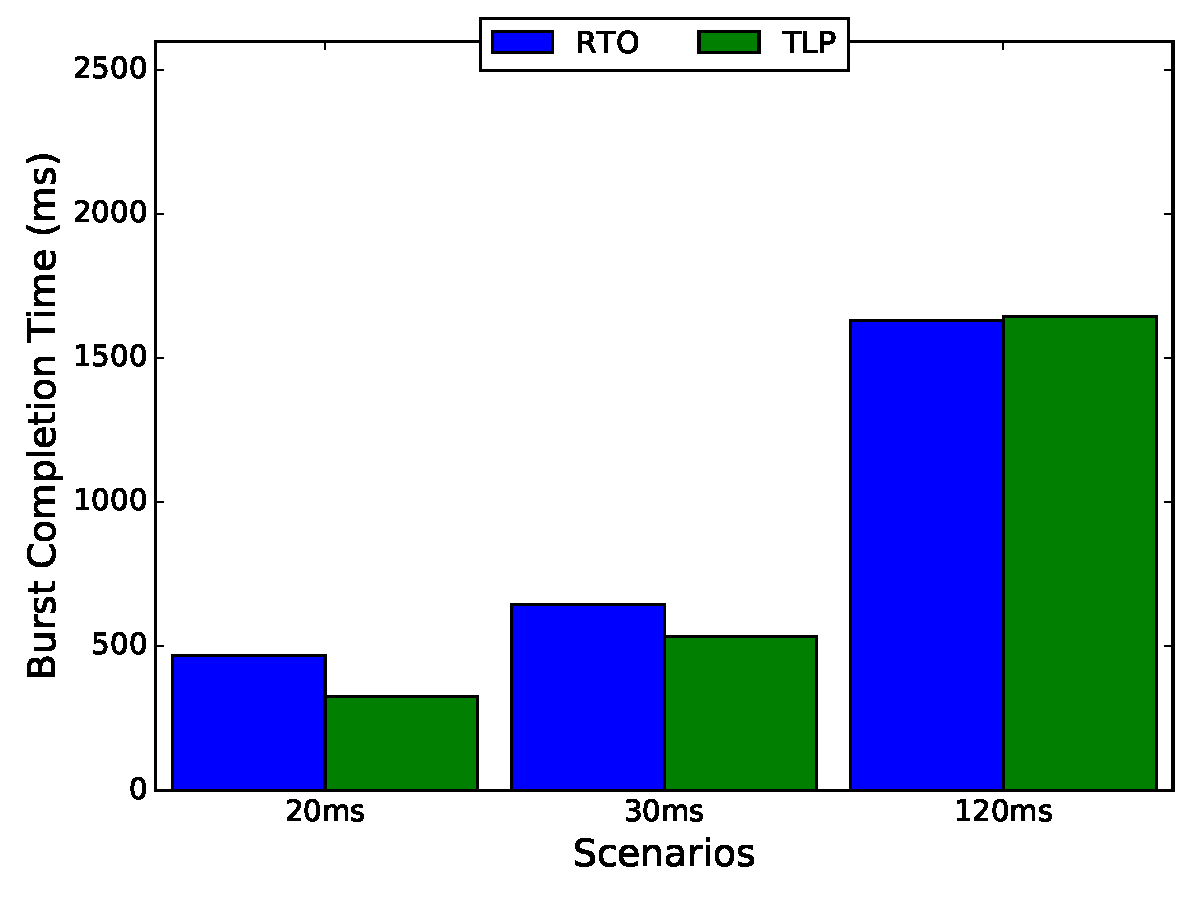
\includegraphics[angle=0, width=\textwidth,natwidth=578.16,natheight=433.62]{plots/T2P.pdf}
	\caption{Two packets }\label{t2p}
 \end{subfigure}
 \hfill
 \begin{subfigure}{0.32\textwidth}
	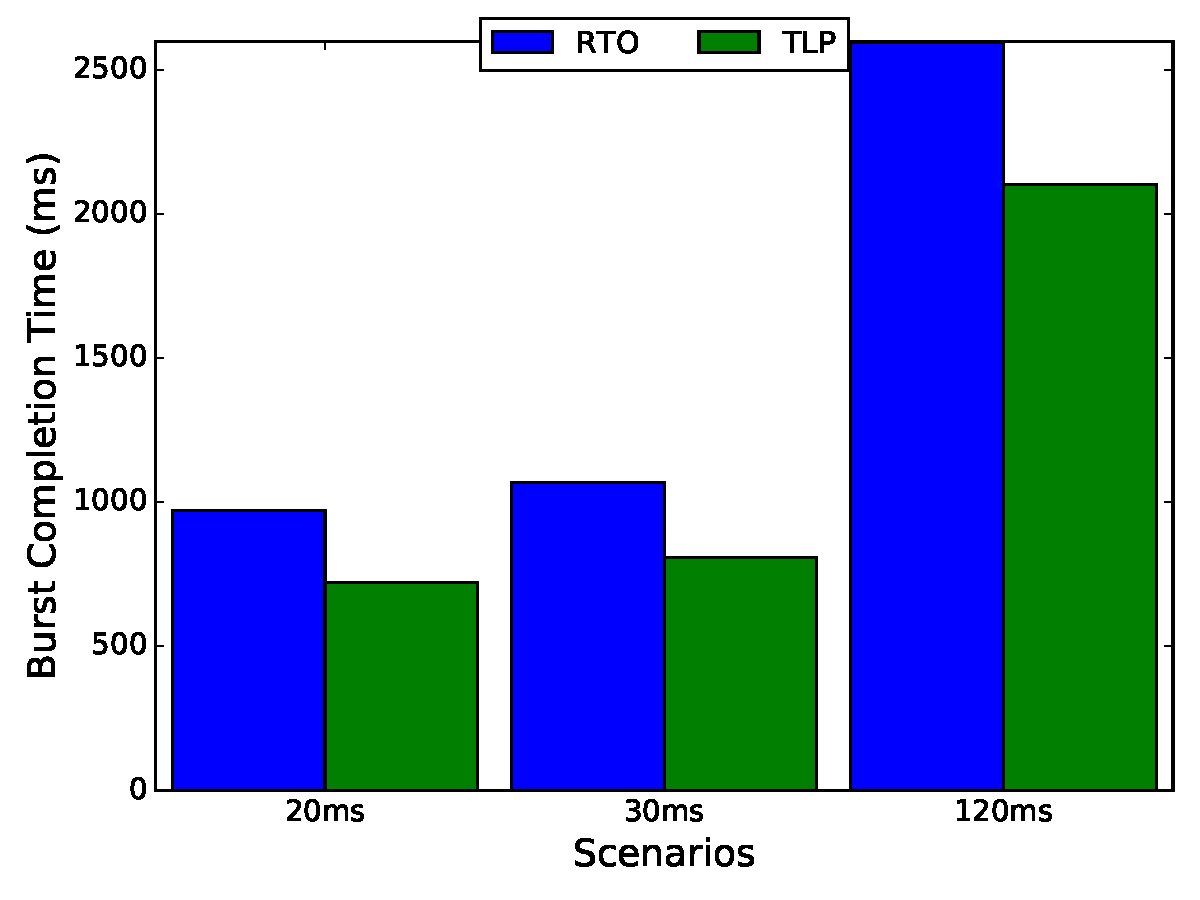
\includegraphics[angle=0, width=\textwidth, natwidth=578.16,natheight=433.62]{plots/T1PP.pdf}
	\caption{Single packet and probe loss }\label{t1pp}
 \end{subfigure}
 \caption{Tail loss scenarios using TCP}\label{tcpf}
\end{figure*}

%\kern-1em
\subsection{Testing retransmission mechanism with deterministic loss patterns}
In order to understand the retransmission behavior of the Linux MPTCP implementation and to reproduce the observed retransmissions, we use a 
deterministic drop pattern. Losses are generated by associating netem with corresponding interfaces and dropping select packets. This process 
is simplified by using the KAUNetem tool~\cite{Garcia2016}, which allows an experimenter to e.g., drop packets based on their positions in a flow. 
A MPTCP connection starts with a single TCP subflow and subsequently, one or more subflows are added following an agreement between the client 
and the server. So one has to wait both in time and packets for the second subflow establishment. We send two bursts of 80 packets each and drop 
tail packets in the second burst at one of the interfaces. This is to ensure that the necessary and sufficient conditions for probe triggering 
are met and tail loss probe is generated on that subflow. We calculate the burst completion time for the second burst that has specified tail 
losses. The objective of this experiment is to evaluate retransmission mechanisms with tail loss (single packet loss and multiple tail loss) and 
temporary path loss. Three test cases are considered for the experiments: single packet tail loss and two packet tail loss for tail loss evaluation 
and single packet along with probe~(in TLP) or retransmission~(in RTO) loss for path loss evaluation. 

In Linux, TCP supports multiple retransmission mechanisms that can be controlled by a system setting. The default setting in Linux enables both
ER and TLP, which may not be the case with other operating systems. In this paper, we use TLP to denote the default Linux setting and RTO to denote
the use of retransmission timeout only.


The setup has server and client with Linux supporting MPTCP running on them. The Client has two interfaces with one way delay on each interface 
ranging from 20\,ms to 120\,ms. The intention is to evaluate the effect of symmetry, mild asymmetry and higher asymmetry in the link delays. We 
consider 5 scenarios with delay pairings 20\,ms-20\,ms, 20\,ms-30\,ms, 20\,ms-120\,ms, 30\,ms-20\,ms, 120\,ms-20\,ms to understand the effect of
delay difference in the performance as shown in Table~\ref{tab1}.


\section{Observations and Discussion}\label{disc}
This section provides the performance analysis of TCP and MPTCP for the considered cases of single packet tail loss, two packet tail loss and 
retransmission or probe loss.
\subsection{TCP}
Retransmission behavior of TCP provides a base case for MPTCP performance as each individual MPTCP subflow is a TCP flow in itself. Our analysis
starts with the results using TCP and compares it with that of MPTCP. Figure~\ref{tcpf} represents the comparison of TCP burst completion times. Path
asymmetry is irrelevant in this case as TCP uses a single path.

In the case of single packet tail loss, as shown in Figure~\ref{t1p}, there is no difference in burst completion between RTO and TLP. The 
retransmission timeout and the probe timeout are the same as there is only one outstanding packet. This is a special case in the TLP
specification that adds 200\,ms to the PTO accommodating the case of delayed ACKs. The TLP implementation in Linux accounts for the delayed 
ACK and waits 200\,ms before sending a probe. The minimum of PTO and RTO is considered for PTO. In the case of two packet tail loss, as shown 
in Figure~\ref{t2p}, TLP performs better than the RTO retransmission for lower delay values. As the delay on the loss path increases RTO retransmission performs 
slightly better than TLP. In 120\,ms case, PTO is very close to RTO expiration and the second packet is recovered using ER which incurs additional 
delay in case of TLP. In RTO retransmission, all unacknowledged packets are retransmitted on a RTO expiration. 

Hence retransmission timeout is the mode of loss recovery in both RTO and TLP. This can be avoided by tuning the ACKs as discussed 
in~\cite{Rajiullah:2015}. In the case of two packet tail loss, TLP performs better than RTO retransmission as it employs a combination of TLP 
and ER to recover from losses. If the probe or retransmission is lost, then TLP still performs better than RTO retransmission as it waits for one 
probe timeout and one RTO experiation instead of two RTO expirations, thus avoiding the exponential backoff of the RTO.

%\kern-1em
\subsection{MPTCP}


The expected retransmission behavior of MPTCP for RTO retransmission and Linux default settings is shown 
in Figure~\ref{mptiming}. The actual pattern might be different in cases where the RTT is larger than 200\,ms. 

\renewcommand{\thesubfigure}{\roman{subfigure}}
\begin{figure*}[!tbp]
 \begin{subfigure}[b]{0.32\textwidth}
	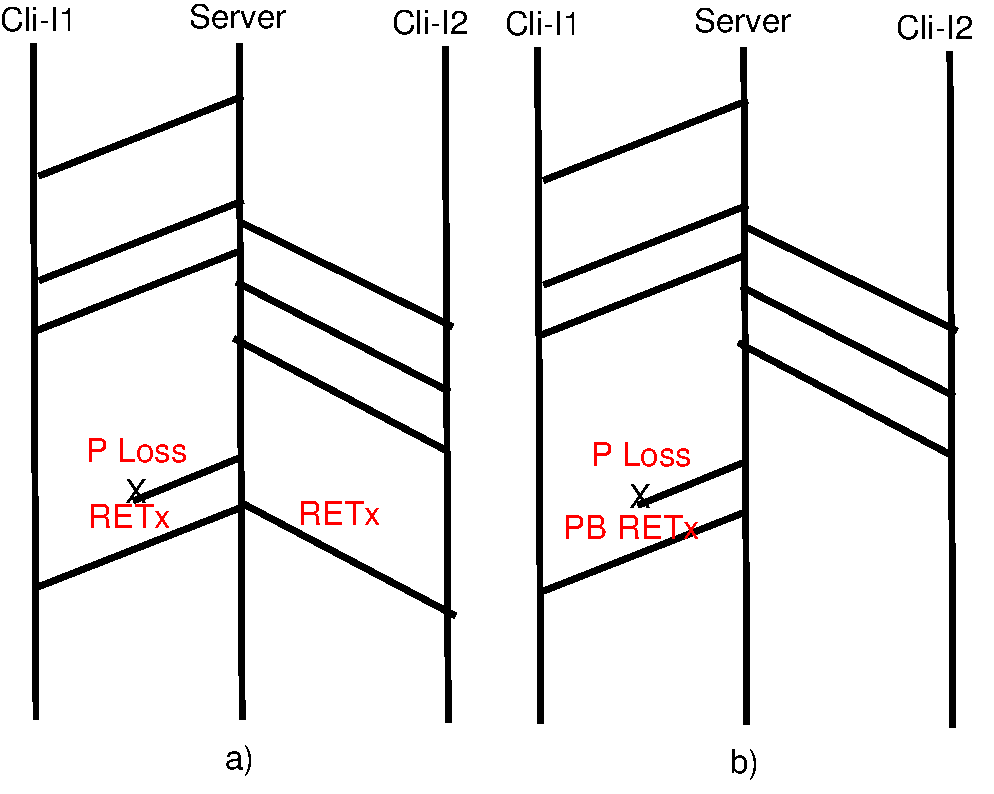
\includegraphics[angle=0, width=\textwidth, natwidth=610, natheight=400]{images/timing1P.pdf}
	\caption{Single packet}\label{timing1P}
 \end{subfigure}
 \hfill
 \begin{subfigure}[b]{0.32\textwidth} 
	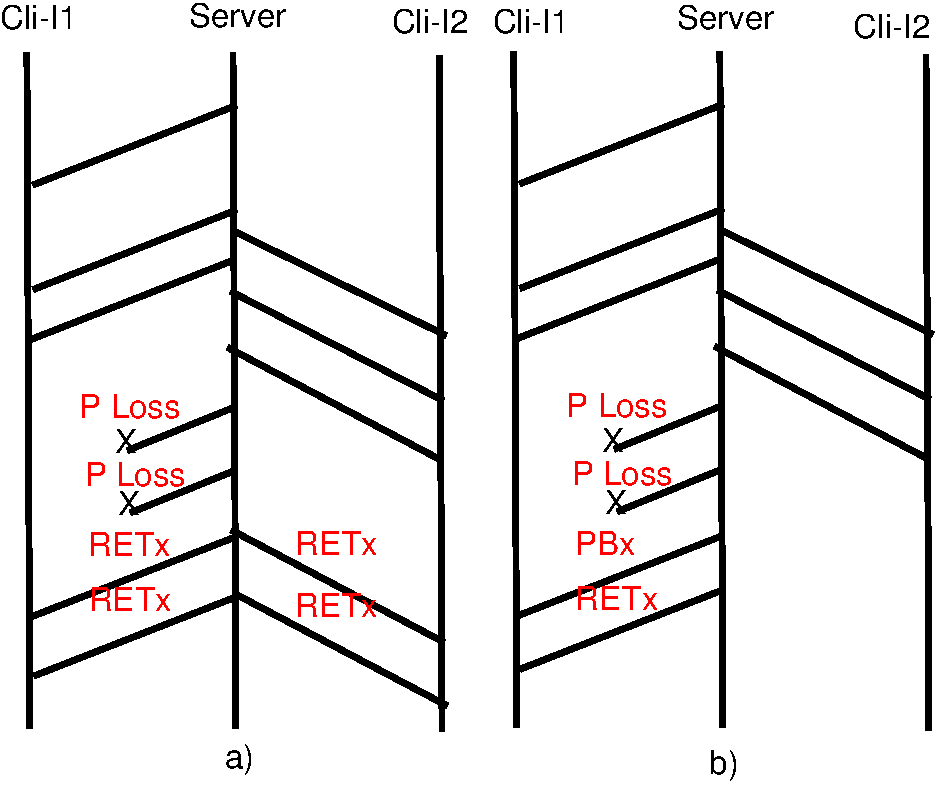
\includegraphics[angle=0, width=\textwidth, natwidth=610, natheight=400]{images/timing2P.pdf}
	\caption{Two packets }\label{timing2P}
 \end{subfigure} 
 \hfill
 \begin{subfigure}[b]{0.32\textwidth}
  	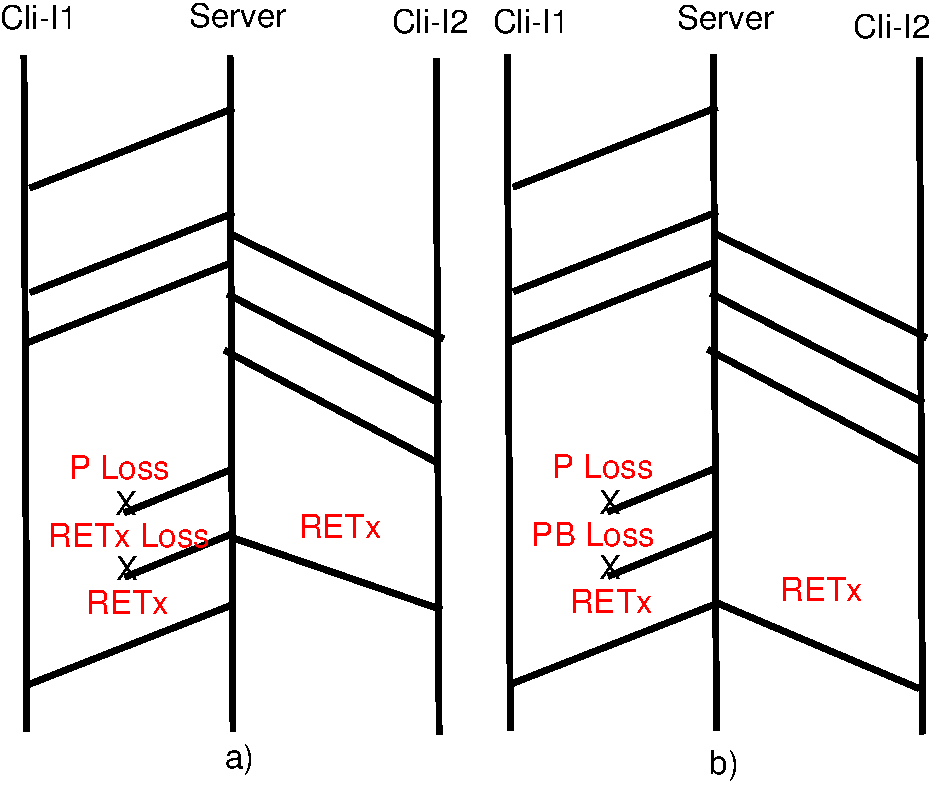
\includegraphics[angle=0, width=\textwidth, natwidth=610, natheight=400]{images/timing1PP.pdf}
	\caption{Single packet and probe loss}\label{timing1PP}
 \end{subfigure}
 \caption{Timing diagrams of MPTCP behavior on tail losses with a) RTO b) TLP }\label{mptiming}	
\end{figure*}


MPTCP uses an RTT based scheduler by default, that uses the lowest RTT path among the available paths to transmit the data until its congestion 
window is full. Subsequently, the next lowest RTT path is chosen. MPTCP performance is sensitive to asymmetry in paths. The burst completion times 
on single packet tail loss calculated for each delay configuration and retransmission setting is depicted in Figure~\ref{1p}. There is no 
difference in performance between RTO retransmission and TLP for cases when both paths are symmetric or the first path has lowest RTT. RTO performs 
better than TLP when the first path is not the lowest RTT path. In such scenarios~(30\,ms-20\,ms,120\,ms-20\,ms), the RTO retransmission happens 
in the second path with lowest RTT following the behavior depicted in Figure~\ref{timing1P}.

\renewcommand{\thesubfigure}{\alph{subfigure}}
\begin{figure*}[!tbp]
 \begin{subfigure}[b]{0.32\textwidth}
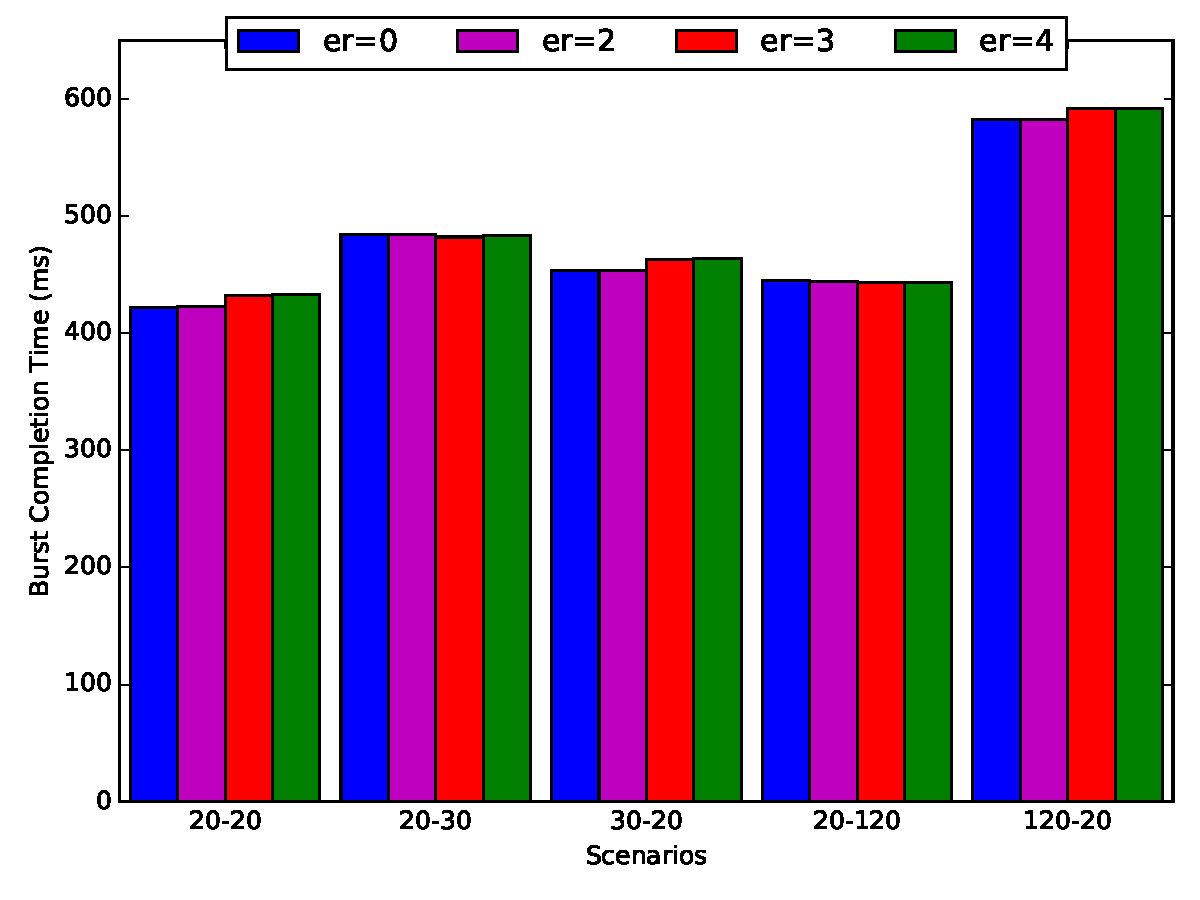
\includegraphics[angle=0, width=\textwidth,natwidth=578.16,natheight=433.62]{plots/1P.pdf}
\caption{Single packet}\label{1p}
 \end{subfigure}
 \hfill
 \begin{subfigure}[b]{0.32\textwidth}
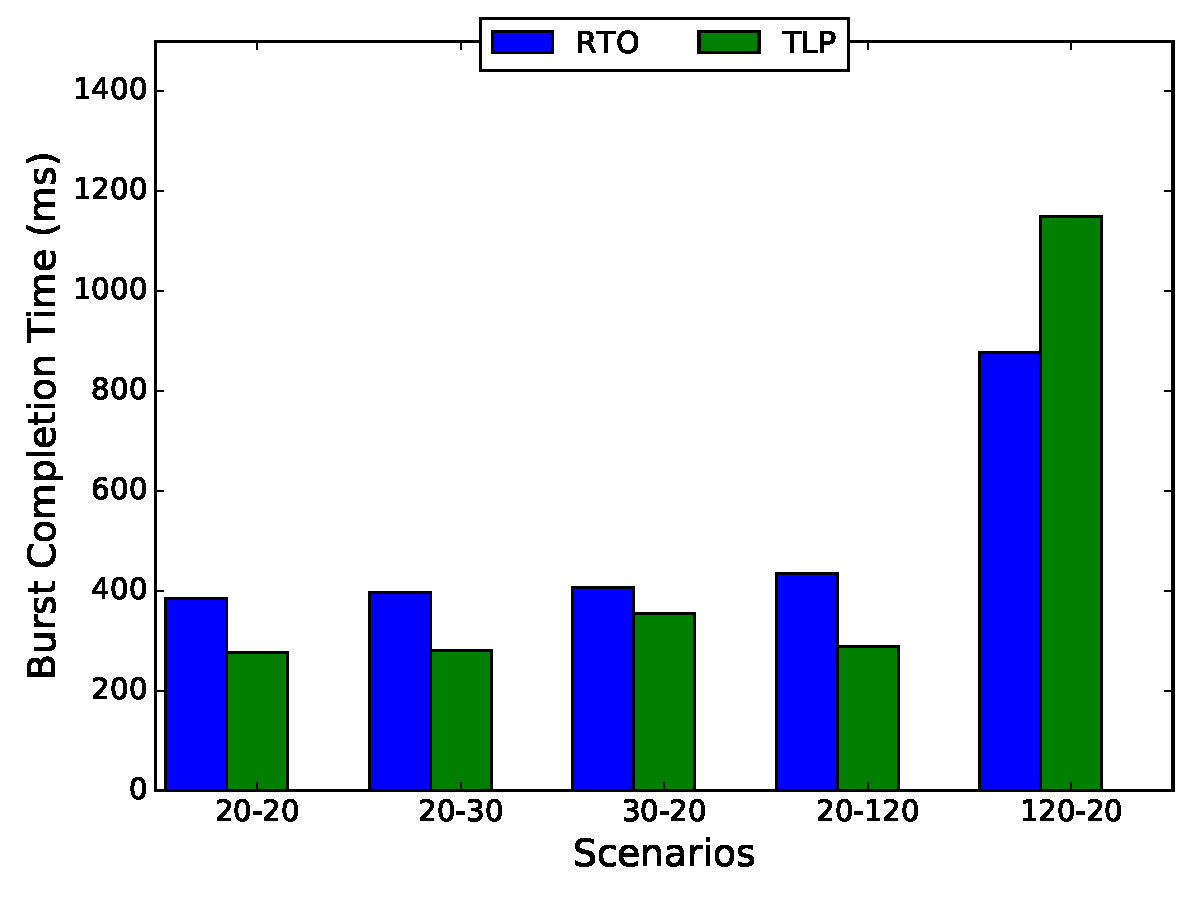
\includegraphics[angle=0, width=\textwidth,natwidth=578.16,natheight=433.62]{plots/2P.pdf}
\caption{Two packets}\label{2p}
 \end{subfigure}
 \hfill
 \begin{subfigure}[b]{0.32\textwidth}
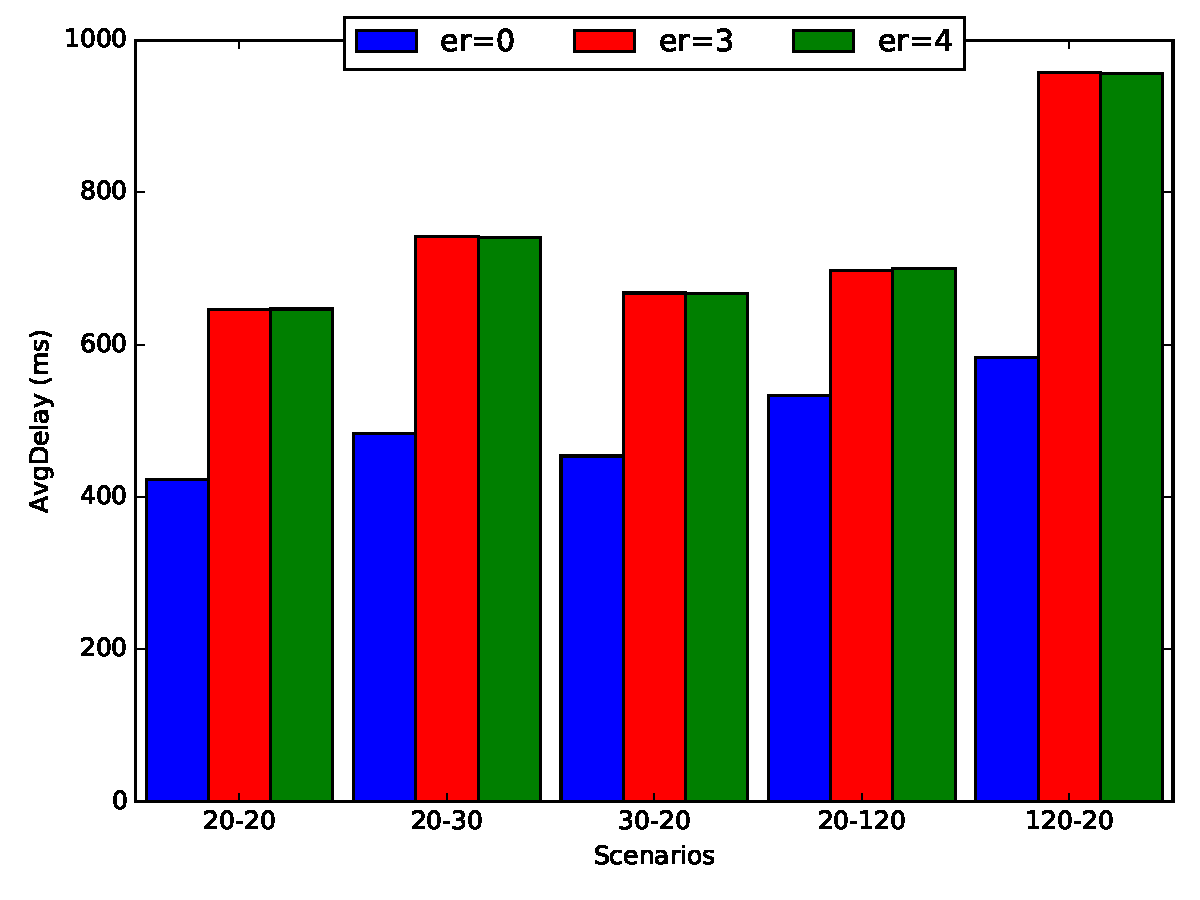
\includegraphics[angle=0, width=\textwidth, natwidth=578.16,natheight=433.62]{plots/1PP.pdf}
\caption{Single packet and probe loss}\label{1pp}
 \end{subfigure}
 \caption{Tail loss scenarios using MPTCP}
\end{figure*}




In the case of single packet tail loss, the last outstanding packet is sent as probe and in case of n-degree tail loss, the latest packet is sent 
as probe to trigger fast retransmit of the packets in between. In order to observe the performance of n-degree tail loss, we consider dropping the 
last two packets. The results of two packet tail loss are shown in Figure~\ref{2p}. In this case, TLP performs better than the other 
two settings in all scenarios except when packets are lost on a high delay interface. In this scenario, the MPTCP retransmission follows the 
behavior depicted in Figure~\ref{timing2P} and the delay difference is large enough that the retransmission of the last packet on the alternate 
path is faster than the probe on the primary path. 


To further study the performance of TLP in the case when there is longer path interruption on one path, we tried to drop the probe packet along 
with the last packet. In this scenario, the RTO setting results in much lower burst completion times. Comparing with the performance of TLP in 
TCP from Figure~\ref{t1pp}, where we saw that use of TLP improved the burst completion time, TLP in MPTCP did not improve the performance. The 
reason lies in the way the retransmission and loss probe transmission is carried out in MPTCP. Retransmission occurs after an RTO time on both 
paths. Even if the retransmission fails on one path, the client receives the packet on the other path as shown in Figure~\ref{timing1PP}. For TLP, 
in the current implementation, the loss probe is sent on the actual path of the first transmission but not on both paths. This incomplete impartation 
of TLP from TCP to MPTCP led to the increase in burst completion time by an RTO for MPTCP. 



%\kern-1em
\section{Improvements to TLP for MPTCP}\label{impr}
The goal of Tail Loss Probe~(TLP) is to reduce tail latency of short flows. It achieves this by converting retransmission timeouts (RTOs) occurring
due to tail losses into fast recovery. TLP transmits one packet in two round-trips when a connection is in Open state and is not receiving any ACKs.
The transmitted packet, or loss probe, can be either new or a retransmission. When there is tail loss, the ACK from a loss probe triggers 
FACK/early-retransmit based fast recovery, thus avoiding a costly retransmission timeout. Our results show that the current TLP implementation for 
MPTCP helps improving the latency performance in cases when the paths are symmetric or the first path~(for the packet) has lowest RTT. However, 
it reduces the performance in cases when the first path is not the lowest RTT path or when there is longer path interruption.

\begin{figure*}
\begin{center}
    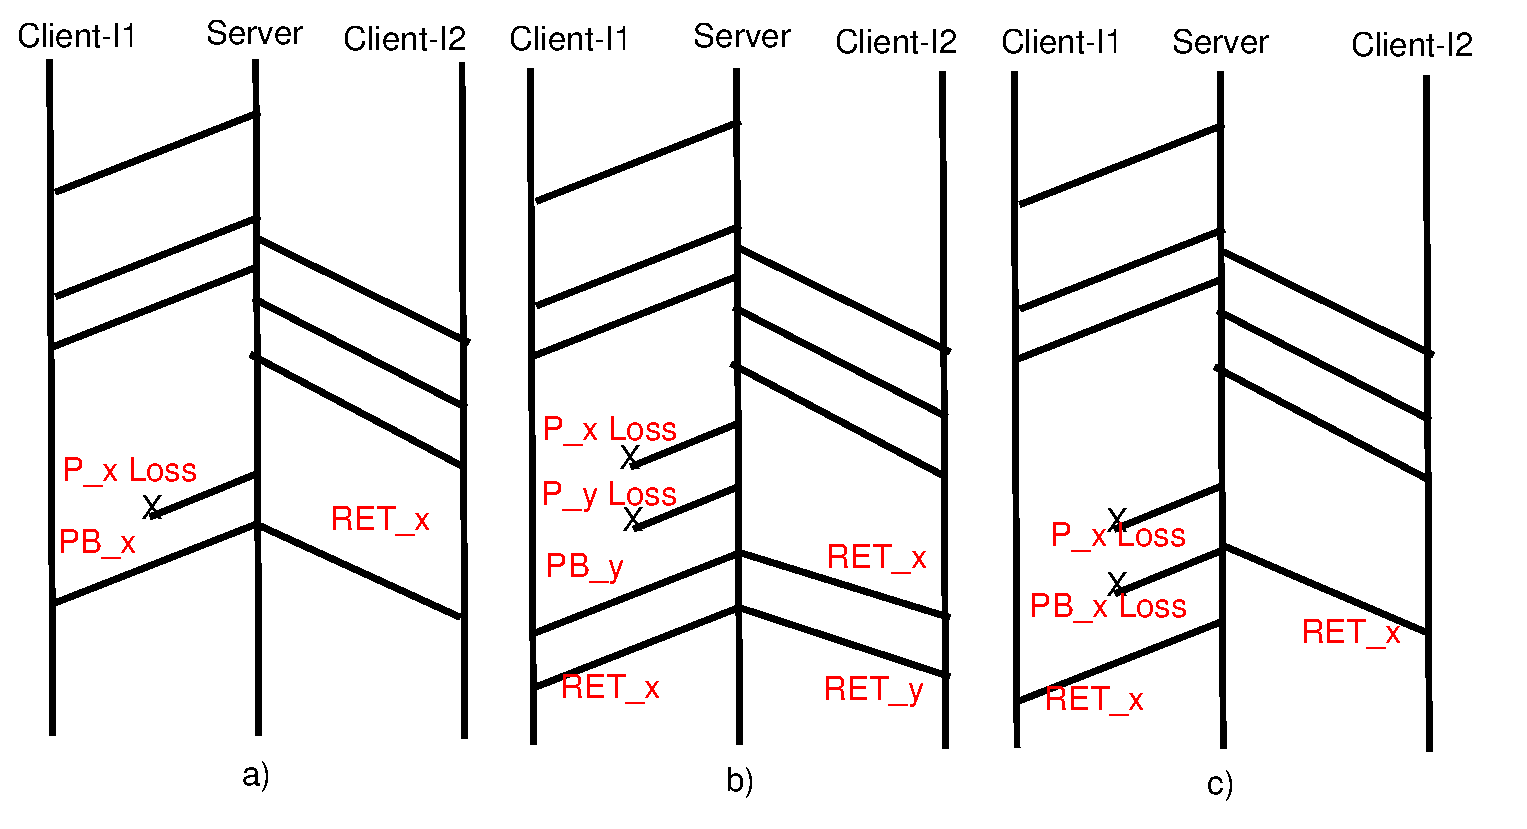
\includegraphics[angle=0, width=0.8\textwidth]{images/timingER3NewTLP1}
\end{center}
\caption{Timing diagram of MPTCP behavior with proposed improvements with loss of a) Single packet b) Two packets c) Single packet and probe loss}\label{timingNew}
\end{figure*}

\begin{figure*}
\begin{subfigure}[b]{0.32\textwidth}
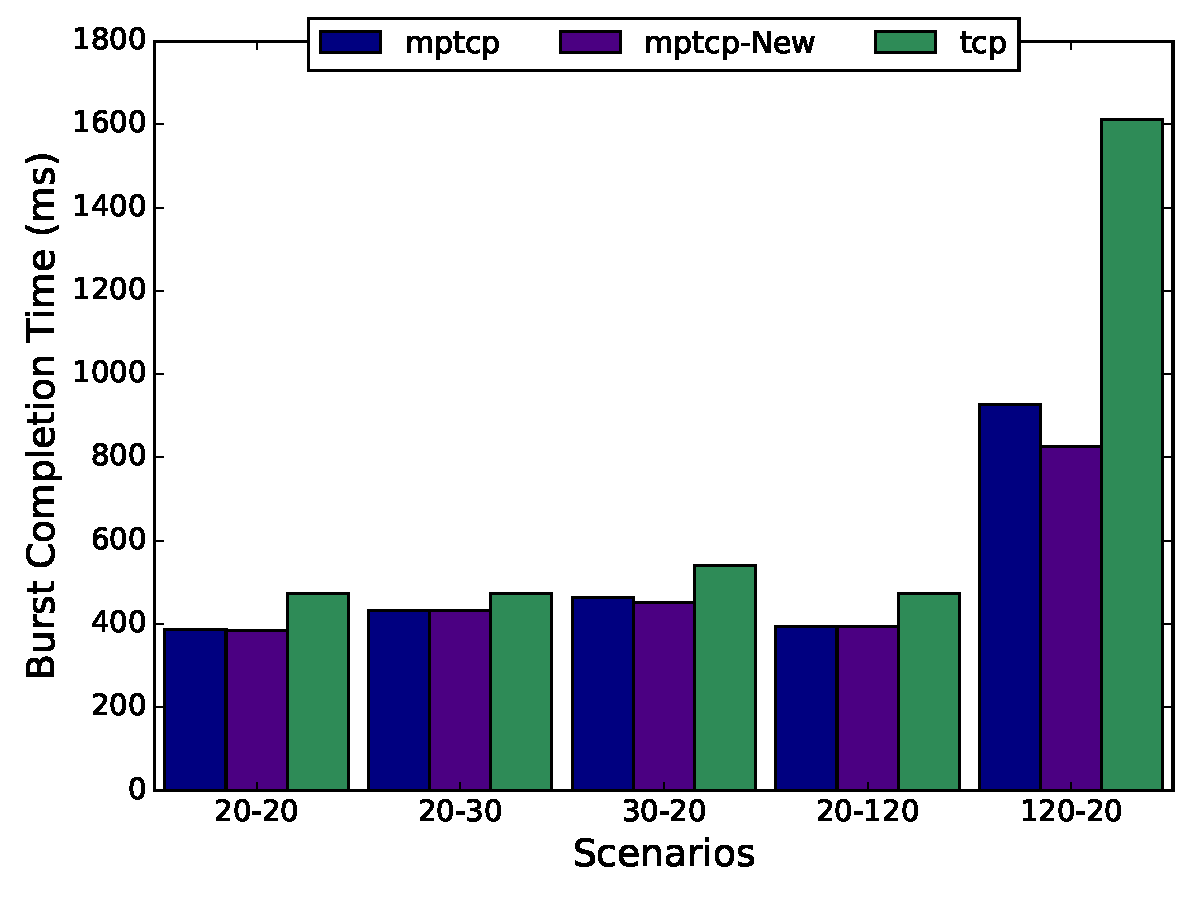
\includegraphics[angle=0, width=\textwidth, natwidth=578.16,natheight=433.62]{plots/1PNew.pdf}
\caption{Single packet}\label{1pn}
\end{subfigure}
\hfill
\begin{subfigure}[b]{0.32\textwidth}
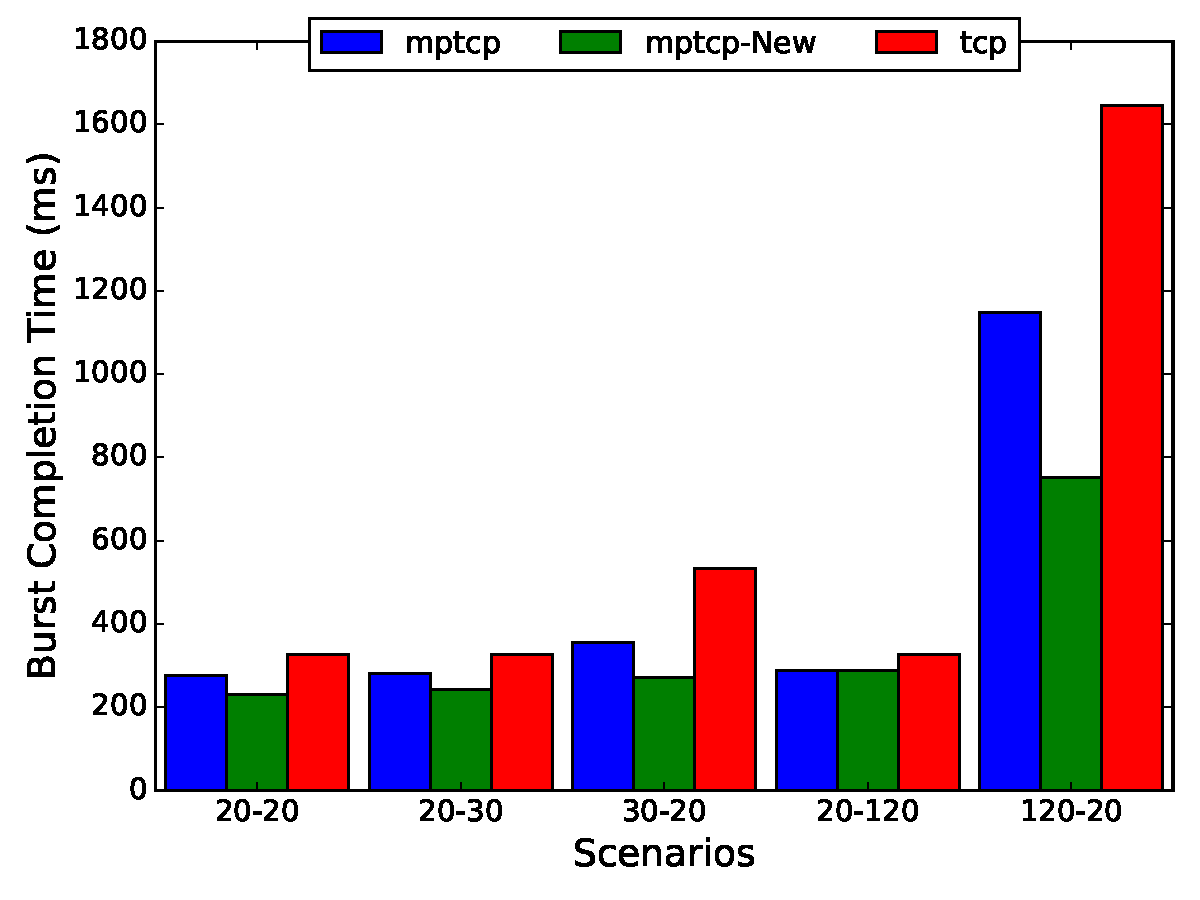
\includegraphics[angle=0, width=\textwidth, natwidth=578.16,natheight=433.62]{plots/2PNew.pdf}
\caption{Two packets}\label{2pn}
\end{subfigure}
\hfill
\begin{subfigure}[b]{0.32\textwidth}
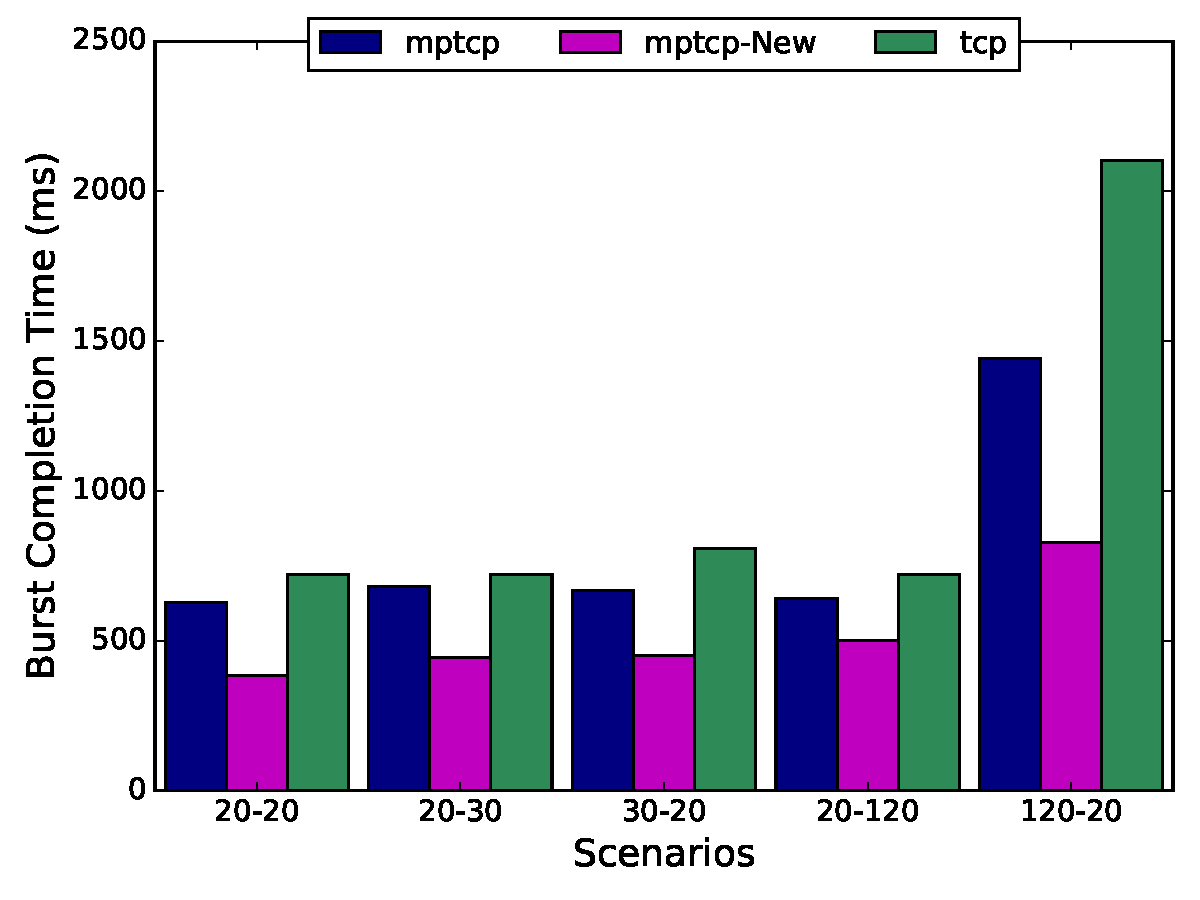
\includegraphics[angle=0, width=\textwidth, natwidth=578.16,natheight=433.62]{plots/1PPNew.pdf}
\caption{Single packet and probe loss}\label{1ppn}
\end{subfigure}
\caption{Performance comparison of MPTCP-New with MPTCP and TCP}\label{mpnew}
\end{figure*}

The current implementation of TLP is at the TCP flow level. In the event of RTO timeout, the MPTCP retransmission happens with a re-injection in 
to the scheduler along with sending the lost packet on the same path. But in the event of Probe timeout, the loss probe packet is being sent on 
the same path without being re-injected in to the scheduler. We propose a modification to the probe sending mechanism for MPTCP by re-injecting 
the probe packet in to the MPTCP scheduler in the event of PTO. As the probe timeout is meant for acting faster than the RTO timeout with 
essentially the same consequence as a retransmission, it is relevant to follow the same process as upon an RTO. It is expected that this 
modification is useful when the alternate path has lower delay than the packet original transmission path or when there is longer path 
interruption. The timing diagram depicted in Figure~\ref{timingNew} indicates the eventual behavior of modified MPTCP TLP for each of the studied 
loss scenarios.




<<<<<<< HEAD
\begin{figure*}[!ht]
\begin{center}
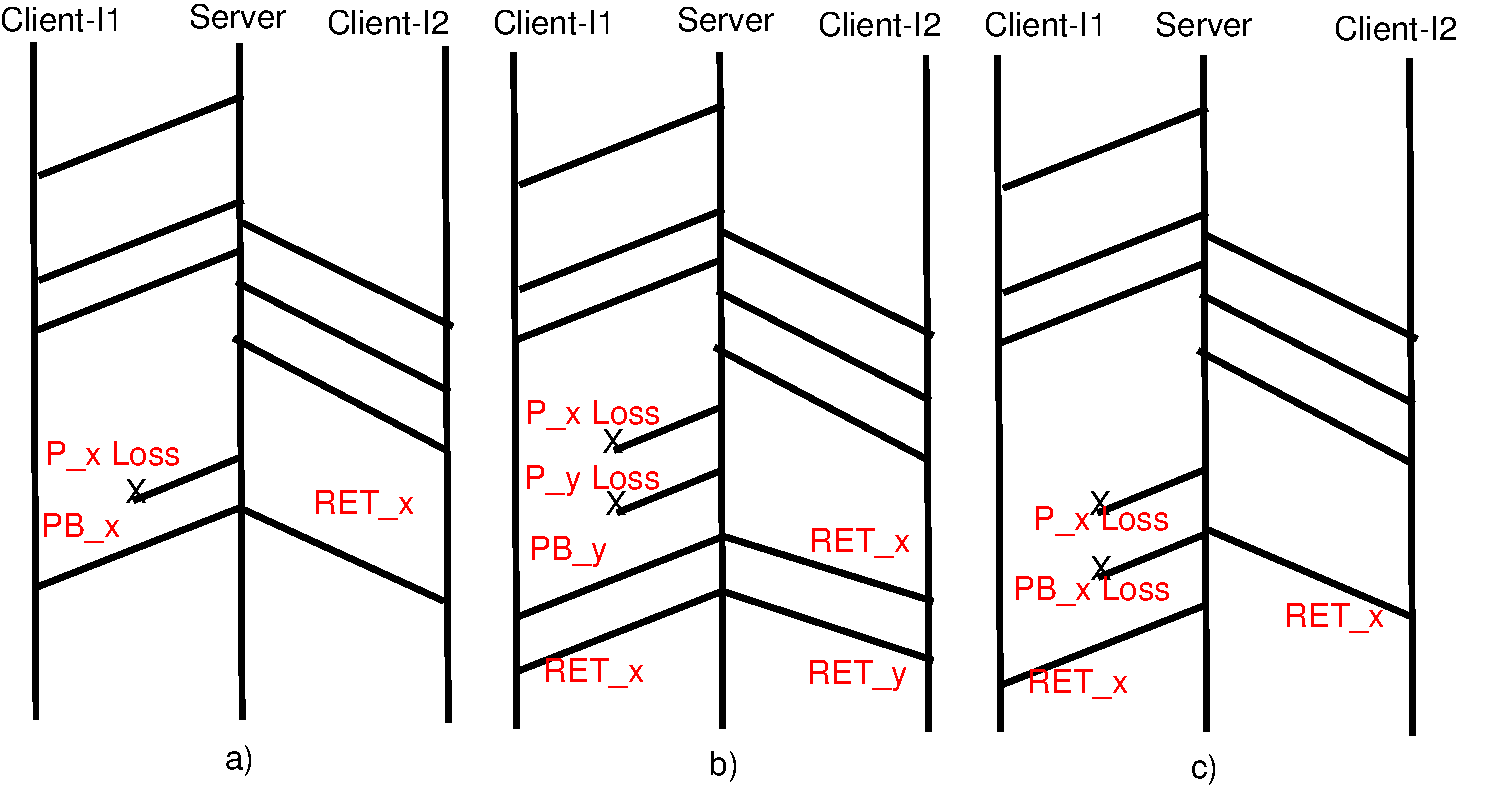
\includegraphics[angle=0, width=\textwidth]{images/timingER3NewTLP1.pdf}
\end{center}
\caption{Timing diagram of MPTCP behavior with proposed improvements with loss of a) Single packet b) Two packets c) Single packet and probe loss}\label{timingNew}
\end{figure*}
=======
>>>>>>> 995f6933bb9382c0c0296a0c955f17863595b3a1

%\kern-1em
\section{Evaluation of modified MPTCP TLP}\label{eval}

Results comparing the burst completion time for new MPTCP TLP with that of TCP and MPTCP TLP for the considered cases are provided in 
Figure~\ref{mpnew}. In Figure~\ref{1pn}, MPTCP-New performs better than TCP in all scenarios, performs equal to MPTCP in symmetric scenarios and 
performs better than MPTCP in asymmetric scenarios with a lower delay on the alternate path. MPTCP-New achieves this improvement by retransmitting
 lost packets on the alternate path much before the RTO. In two packet tail loss scenario as in Figure~\ref{2pn}, MPTCP-New
performs better than TCP in all scenarios and better than MPTCP in all scenarios except when the alternate path has a significantly higher delay 
than the original path, where performance is the same. In the single packet together with probe loss scenario as in Figure~\ref{1ppn}, MPTCP-New 
performs better than both MPTCP and TCP in all scenarios with PTO triggering the probe retransmission on alternate path much earlier than the RTO.


%\kern-1em
\section{Conclusions}\label{conc}
This paper provides a short comparative analysis of retransmission behavior with TCP and MPTCP protocols using various loss patterns for tail loss.
The three cases of tail loss together with deterministic loss patterns allow us to dissect the retransmission behavior at packet level to 
understand possible improvements.
We propose a less conservative approach to trigger retransmission on an alternate path in the event of tail loss probe timeout, which otherwise 
triggered with an RTO. Our emulation experiments  using a modified Linux implementation, show that the proposed approach in fact improves the 
burst completion time in most cases and equals the existing implementation in other cases. The proposed approach improves the performance when 
the alternate path has lower delay than the original loss path and the advantage increases with degree of asymmetry between the paths. 
Temporary path failures can cause probe loss along with packet loss. The approach is very effective in case of probe loss which otherwise 
incur RTO timeout to trigger retransmission on either path. However, the latency improvement comes at a cost of additional network traffic 
from the retransmitted packets. This study is limited to emulated synthetic traffic and static drop pattern that serve the purpose of localizing 
the loss events. A comprehensive study covering various traffic types and loss patterns is considered for future investigation. Further, we plan 
to investigate less conservative approaches for other retransmission events.

\section*{Acknowledgment}
This work was in part funded by The Knowledge Foundation (KKS) through the SIDUS READY project. The views expressed are solely those of the 
author(s).
   
%\kern-1em
\bibliographystyle{IEEEtran}
\bibliography{mptcp-retrans}
\end{document} 
